% \section{Phân tích và tiền xử lý dữ liệu}

% \subsection{Bộ dữ liệu: FoodSeg103}

% \begin{figure}[H]
%     \centering
%     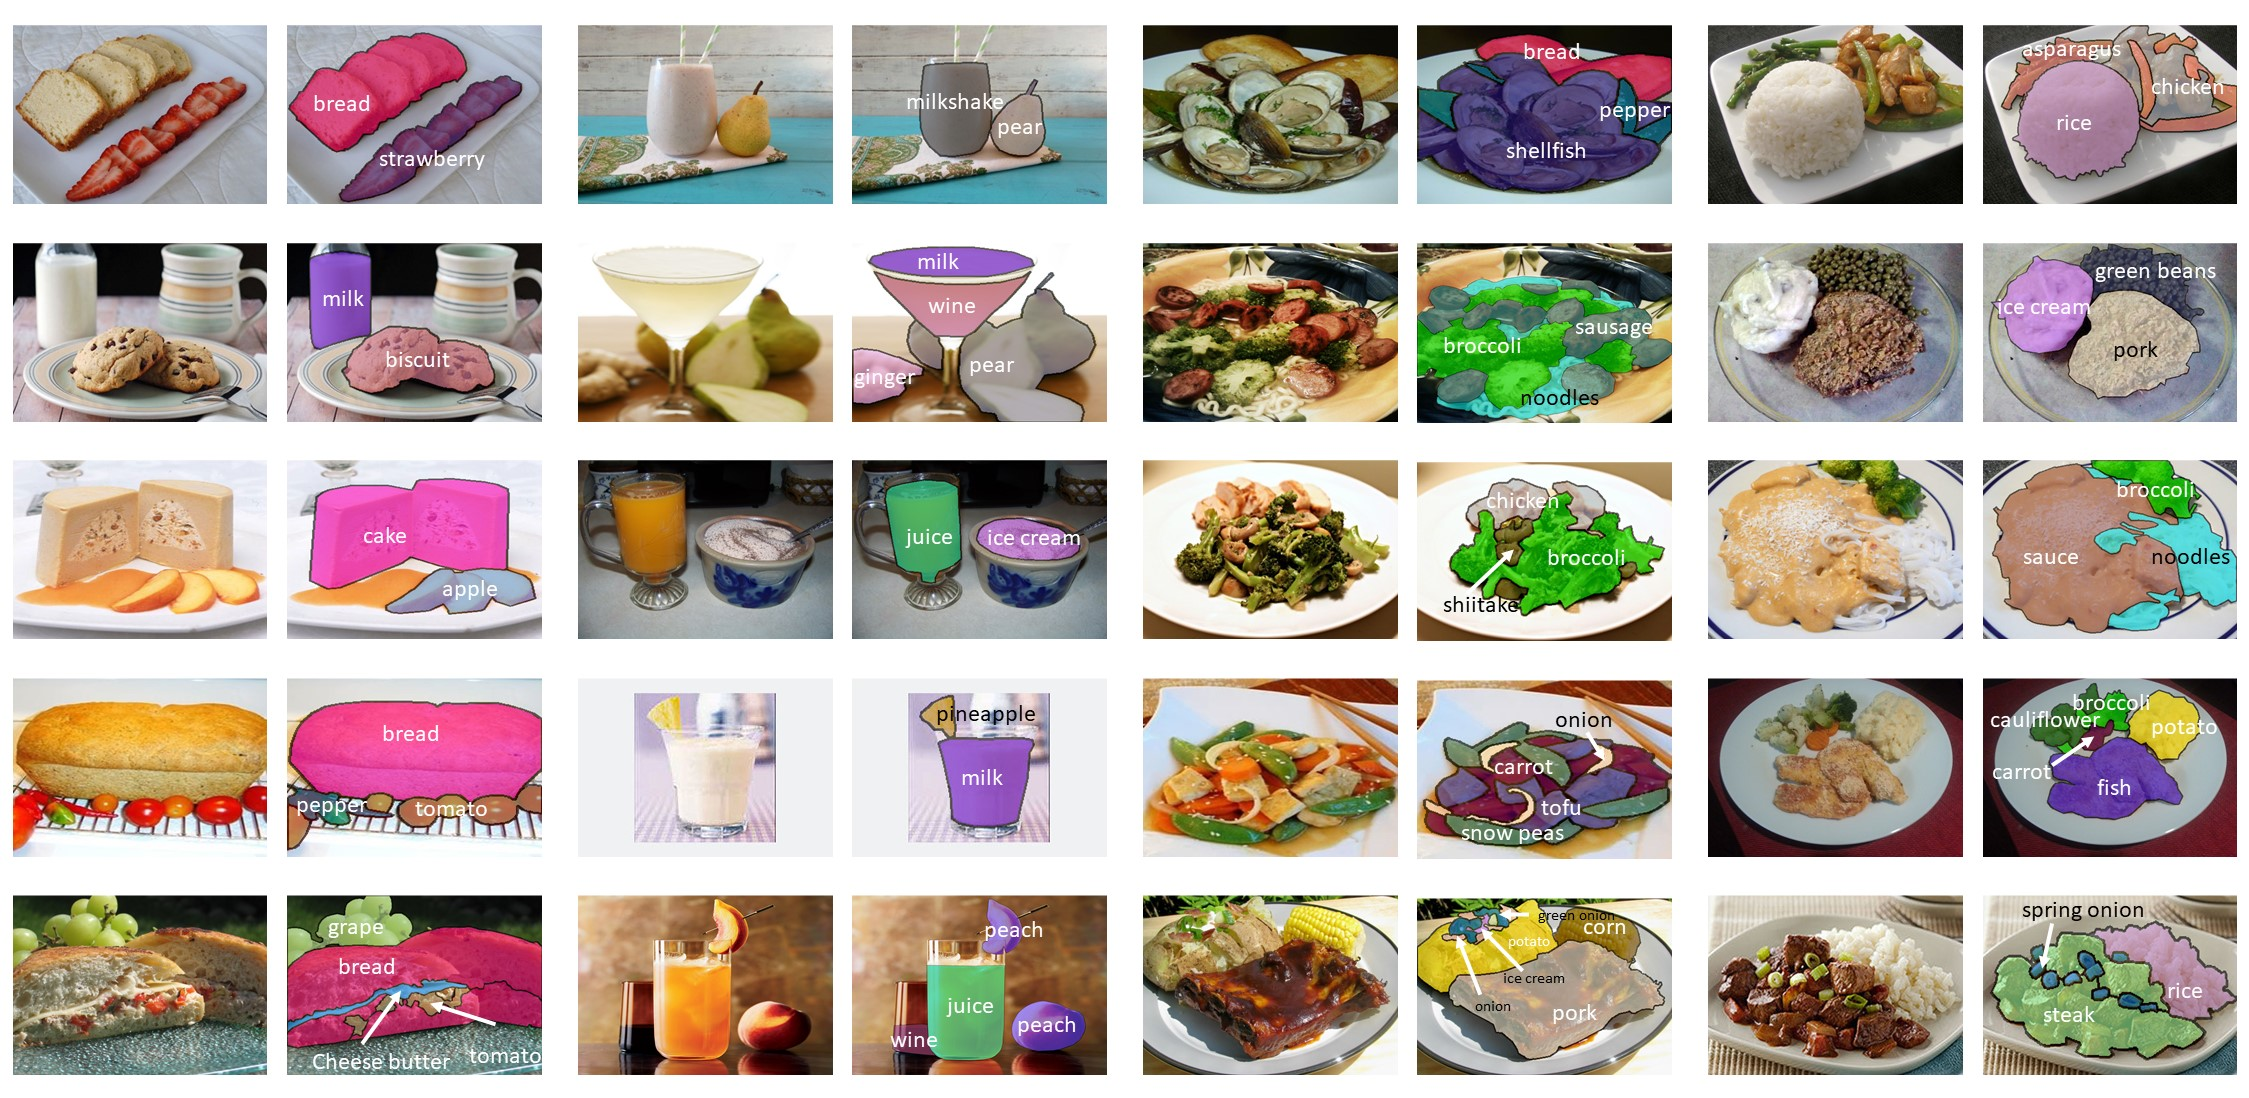
\includegraphics[width=\linewidth]{img/foodseg103.png}
%     \caption{Mẫu ảnh đại diện cho một số lớp trong bộ dữ liệu FoodSeg103, thể hiện sự đa dạng về kết cấu và màu sắc.}
% \end{figure}

% FoodSeg103 là một trong những bộ dữ liệu chuẩn mực quy mô lớn đầu tiên được thiết kế chuyên biệt cho bài toán phân vùng hình ảnh thức ăn ở cấp độ nguyên liệu. Bộ dữ liệu này được giới thiệu bởi Wu và cộng sự tại hội nghị ACM Multimedia 2021, thông qua việc chắt lọc và gán nhãn thủ công từ Recipe1M - một kho dữ liệu khổng lồ chứa hàng triệu hình ảnh và công thức nấu ăn \cite{benchmarkfood}. Khác với các bộ dữ liệu trước đây thường chỉ giải quyết bài toán phân loại vùng có món ăn, FoodSeg103 đi sâu vào chi tiết của từng thành phần nguyên liệu cấu tạo nên món ăn đó.

% Tập dữ liệu gồm tổng cộng 6117 ảnh, trong đó có 3982 ảnh huấn luyện và 2135 ảnh kiểm thử. Kích thước ảnh trung bình của train là $770.80\times640.58$ pixel, lớn hơn đáng kể so với test ở mức $578.80\times480.01$ pixel. Sự khác biệt về kích thước này dễ dẫn đến hiện tượng \emph{domain gap} do độ phân giải, làm suy giảm độ tin cậy của mô hình nếu dữ liệu không được tiền xử lý và chuẩn hóa nhất quán trên cả hai tập (split).

% % \begin{figure}[H]
% %     \centering
% %     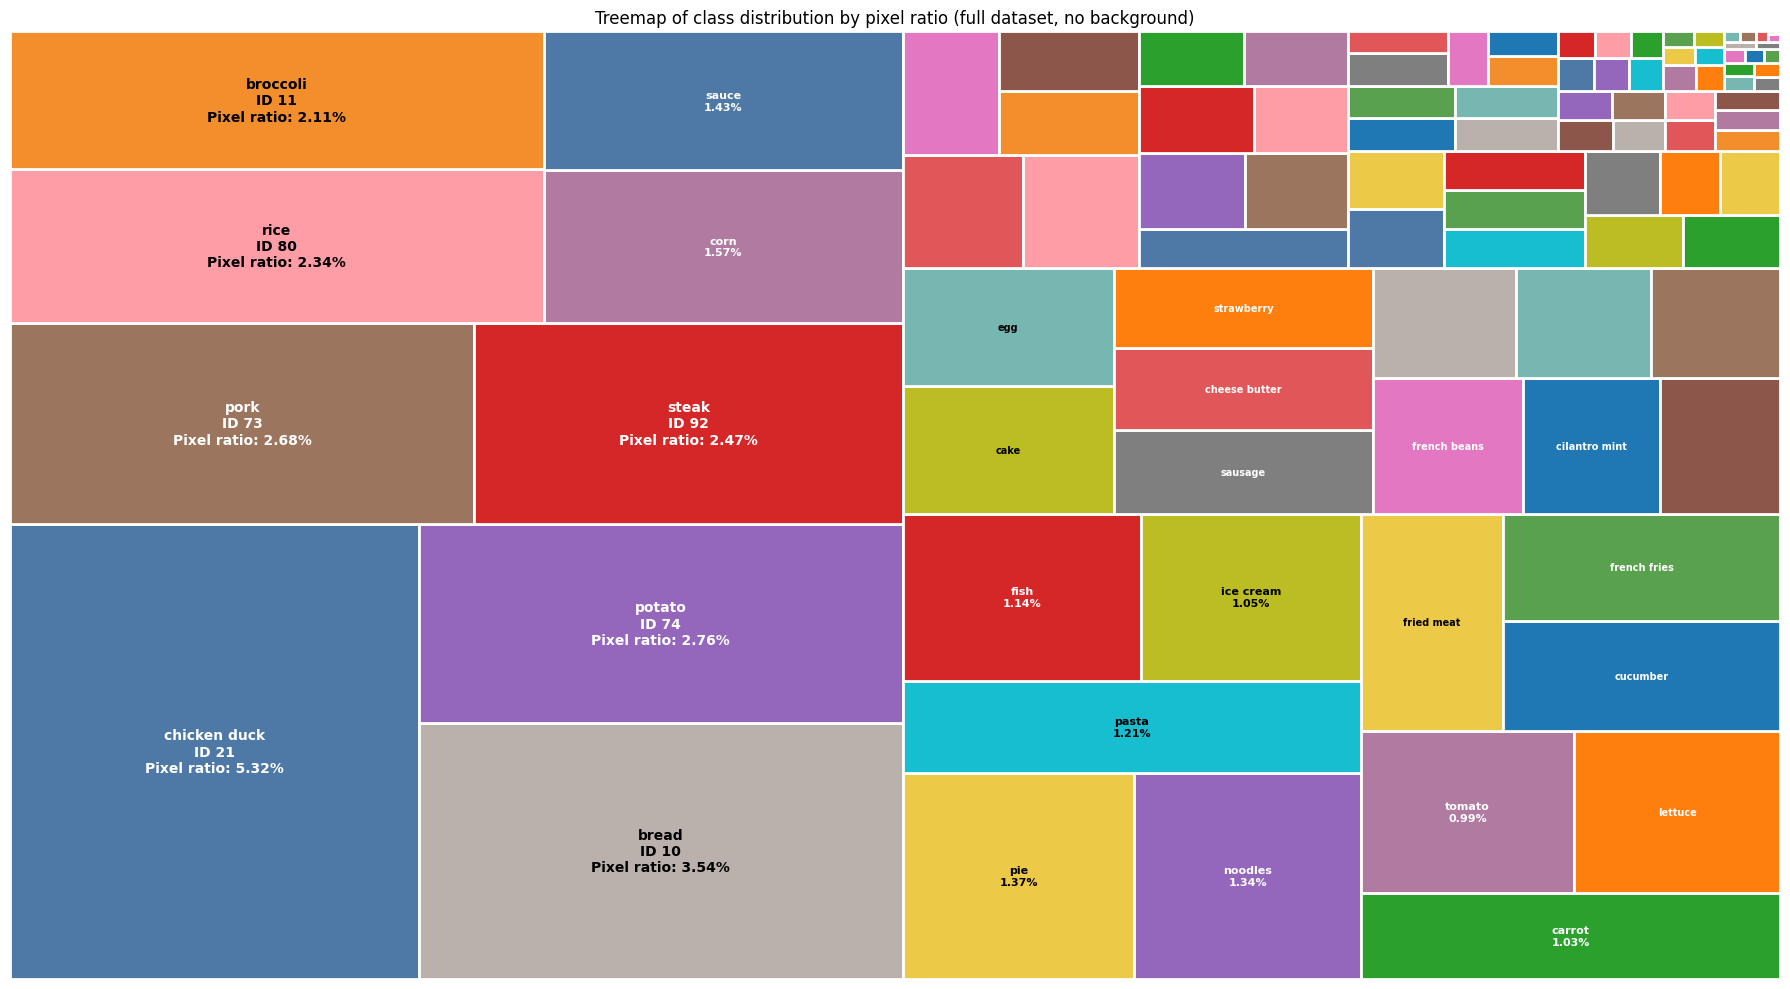
\includegraphics[width=\linewidth]{img/analyze/tree-map.png}
% %     \caption{Sự phân bố số lượng ảnh theo lớp trên bộ dữ liệu gốc.}
% % \end{figure}


% Về độ toàn vẹn, bộ dữ liệu đạt chất lượng gần như tuyệt đối với tỷ lệ ảnh hợp lệ trên 99.97\% ở cả hai tập và bao phủ đầy đủ toàn bộ 103 lớp foreground được định nghĩa trong metadata.

% \begin{table}[H]
%     \centering
%     \caption{Toàn vẹn dữ liệu trên bộ dữ liệu gốc}
%     \begin{tabular}{lrrr}
%         \toprule
%         Split & Ảnh hợp lệ & Tổng ảnh & Tỉ lệ hợp lệ \\
%         \midrule
%         Train & 3981 & 3982 & 99.97\% \\
%         Test  & 2135 & 2135 & 100.00\% \\
%         \bottomrule
%     \end{tabular}
% \end{table}

% Vấn đề đáng chú ý nhất của bộ dữ liệu là sự phân bố đuôi dài nghiêm trọng. Theo thống kê mức bao phủ pixel, các lớp phổ biến như \texttt{chicken duck} và \texttt{bread} chiếm lần lượt 4.91\% và 3.34\% tổng số pixel, trong khi các lớp hiếm như \texttt{bamboo shoots} và \texttt{kelp} gần như bằng 0 (xấp xỉ 0.0004\%). Về mặt vật thể, nhóm phổ biến xuất hiện hơn 1100 lần, bỏ xa các lớp còn lại. Do đó, nếu không có chiến lược tái cấu trúc không gian nhãn, mô hình sẽ rơi vào trạng thái thiên lệch, chỉ tối ưu hóa tốt cho nhóm chiếm đa số nhưng lại thất bại trong việc phân vùng nhóm thiểu số.


